\documentclass[final]{beamer}
\usepackage{multimedia}
\usepackage{color}
\usepackage[normalem]{ulem}
\usepackage{adjustbox}
\graphicspath{{figures/}}

\newcommand{\comment}[1]{}
\definecolor{grigio}{rgb}{.8, .8, .8}

\mode<beamer>{%
	\usetheme{default}
  \usecolortheme{default}
}
\titlegraphic{
\includegraphics[width=0.3\textwidth]{LogoUPF_CBC}\hspace{0.5cm}
\includegraphics[width=0.3\textwidth]{logo_italian_academy}\hspace{0.5cm}
\includegraphics[width=0.15\textwidth]{columbia}}
\title[Effective connectivity]{\textbf{Whole brain effective connectivity from fMRI data}\\ Some subtitle}
\author{Andrea Insabato}
\date{November 27th, 2017}

\begin{document}


\begin{frame}<handout:0>
  \titlepage
\end{frame}

\begin{frame}
\transdissolve
\frametitle{Whole brain connectivity}
\begin{columns}
\begin{column}{0.5\textwidth}
	\begin{itemize}
			\pause
		\item Whole brain is divided in ROIs (parcellation)
			\pause
		\item Average activity in each ROI
			\pause
		\item Connectivity between ROIs
	\end{itemize}
\end{column}
\begin{column}{0.5\textwidth}
\includegraphics<1->[width=0.5\columnwidth,valign=t]{brain_connectivity}
\end{column}
\end{columns}
\end{frame}

\begin{frame}
\transdissolve
\frametitle{Functional Connectivity (FC)}
\begin{columns}
\begin{column}{0.5\textwidth}
\includegraphics<1->[width=0.5\columnwidth,valign=t]{FC}
\end{column}
\begin{column}{0.5\textwidth}
	\begin{itemize}
			\pause
		\item Pearson correlation between ROIs
			\pause
		\item Dense 
			\pause
		\item Symmetric: no directionality of interactions 
	\end{itemize}
\end{column}
\end{columns}
\end{frame}

\begin{frame}
\transdissolve
\frametitle{Effective Connectivity (EC)}
\begin{columns}
\begin{column}{0.5\textwidth}
\includegraphics<1->[width=0.5\columnwidth,valign=t]{EC}
\end{column}
\begin{column}{0.5\textwidth}
	\begin{itemize}
			\pause
		\item Network model 
			\pause
		\item Sparse 
			\pause
		\item Asymmetric: no directionality of interactions 
	\end{itemize}
\end{column}
\end{columns}
\end{frame}

\begin{frame}
\transdissolve
\frametitle{Outline}
\begin{itemize}
		\pause
	\item Network model
		\pause
	\item EC based subject and condition identification
		\pause
	\item Estimation of model parameters
\end{itemize}
\end{frame}

\begin{frame}
\transdissolve
\frametitle{Network model}
\begin{itemize}
		\pause
	\item Each node is an Ornstein-Uhlenbeck process 
		\pause
	\item $dx_i(t) = [-\frac{x_i(t)}{\tau_i} + \sum_{j\ne i} C_{ij} x_j + \eta_i]dt + dB_i;\qquad dB_i\sim\mathcal{N}(0,\sigma_i^2)$ 
		\pause
\end{itemize}
\end{frame}

\begin{frame}
\frametitle<1>{Characterization of whole brain networks underlying ``mental'' states}
\frametitle<2>{Characterization of whole brain networks underlying watching a movie}
\frametitle<3>{Characterization of whole brain networks underlying remembering}
\frametitle<4>{Characterization of whole brain networks underlying calculating}
\frametitle<5>{Characterization of whole brain networks underlying pathological states (dementia, autism, depression, etc.)}
\frametitle<6->{Characterization of whole brain networks underlying ``mental'' states}
\transdissolve
\begin{itemize}
	\item<7-> Separate different sources of varibility
	\visible<9->{
	\begin{itemize}
		\item classify subjects
		\item classify conditions 
		\item extract networks underlying each classification
	\end{itemize}
	}
\end{itemize}
\begin{center}
	\visible<8->{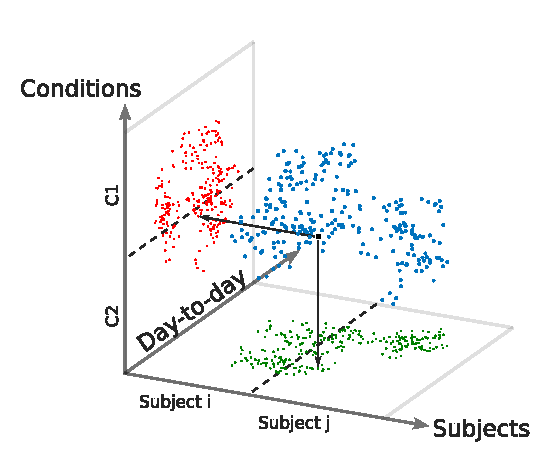
\includegraphics[width=0.5\columnwidth,valign=b]{subj_cond_idea}}
\end{center}
\end{frame}

\begin{frame}
\transdissolve
\frametitle{Datasets}
	\centering
\adjustbox{max width=\textwidth}{
\begin{table}[t!]
\begin{tabular}{l||l|l|l|l}
Dataset name	& Acquisition	 & Number of subjects	 & Sessions per subject	 & Session duration \\
\hline
\hline
Dataset A1	& Day2day project				 & 6			 & 40-50		 & 5 minutes \\
Dataset B	& CoRR						 & 30			 & 10			 & 10 minutes \\
Dataset C	& Gilson et al. 2017, Mantini et al. 2012	 & 19			 & 3 resting; 2 movie	 & 10 minutes \\
\end{tabular}
\end{table}
}
\end{frame}

\begin{frame}
\transdissolve
\frametitle{Subjects classification}
\begin{itemize}
		\pause
	\item Finn (Nat. Neuro. 2015): FC of $\sim100$ subjects, 5 sessions per subject, Nearest Neighbor, 54-94\% accuracy   
		\pause
	\item Our approach:
		\pause
		\begin{itemize}
	\item Comparison between FC and EC
		\pause
	\item Multinomial logistic regression (interpretability of fitted classifier)
		\pause
	\item \textbf{Test-retest} dataset (10-50 sessions per subject): 
		\pause
		\begin{itemize}
			\item accurate assessment of test accuracy 
		\pause
			\item impact of training set size
		\end{itemize}
		\end{itemize}
\end{itemize}
\end{frame}

\begin{frame}
\transdissolve
\frametitle{Multinomial Logistic Regression (MLR)}
\begin{itemize}
	\item $C_k = \sigma(\sum_j^N \beta_{jk} x_j)$
\pause
\item allows to estimate the most relevant features for the classification
	\item Recursive feature elimination: 
		\begin{itemize}
			\item recursively remove feature $i = \operatorname*{arg\,min}_j \sum_k \beta_{jk}$
			\item survival time reflects relevance of each link
		\end{itemize}
\end{itemize}
\end{frame}

\begin{frame}
\frametitle{Subjects classification}
\begin{center}
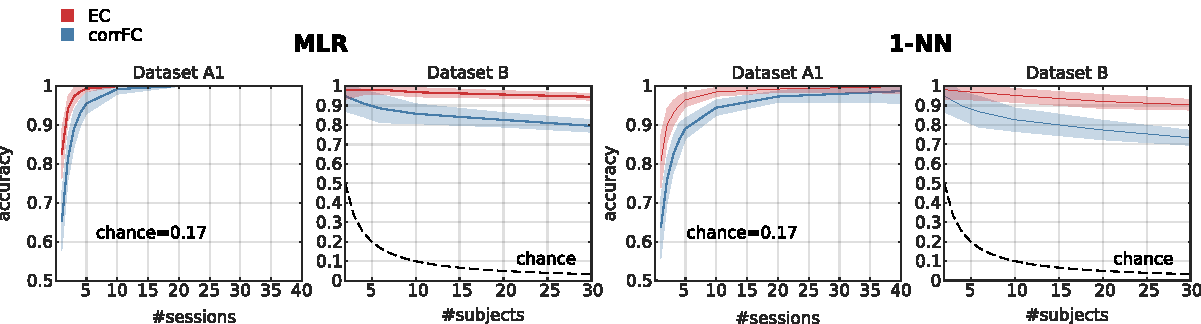
\includegraphics[width=0.9\columnwidth,valign=b]{class_subj}
\end{center}
\end{frame}

\begin{frame}
\frametitle{Subjects classification}
Classification accuracy using subsets of links according to RFE ranking
\begin{center}
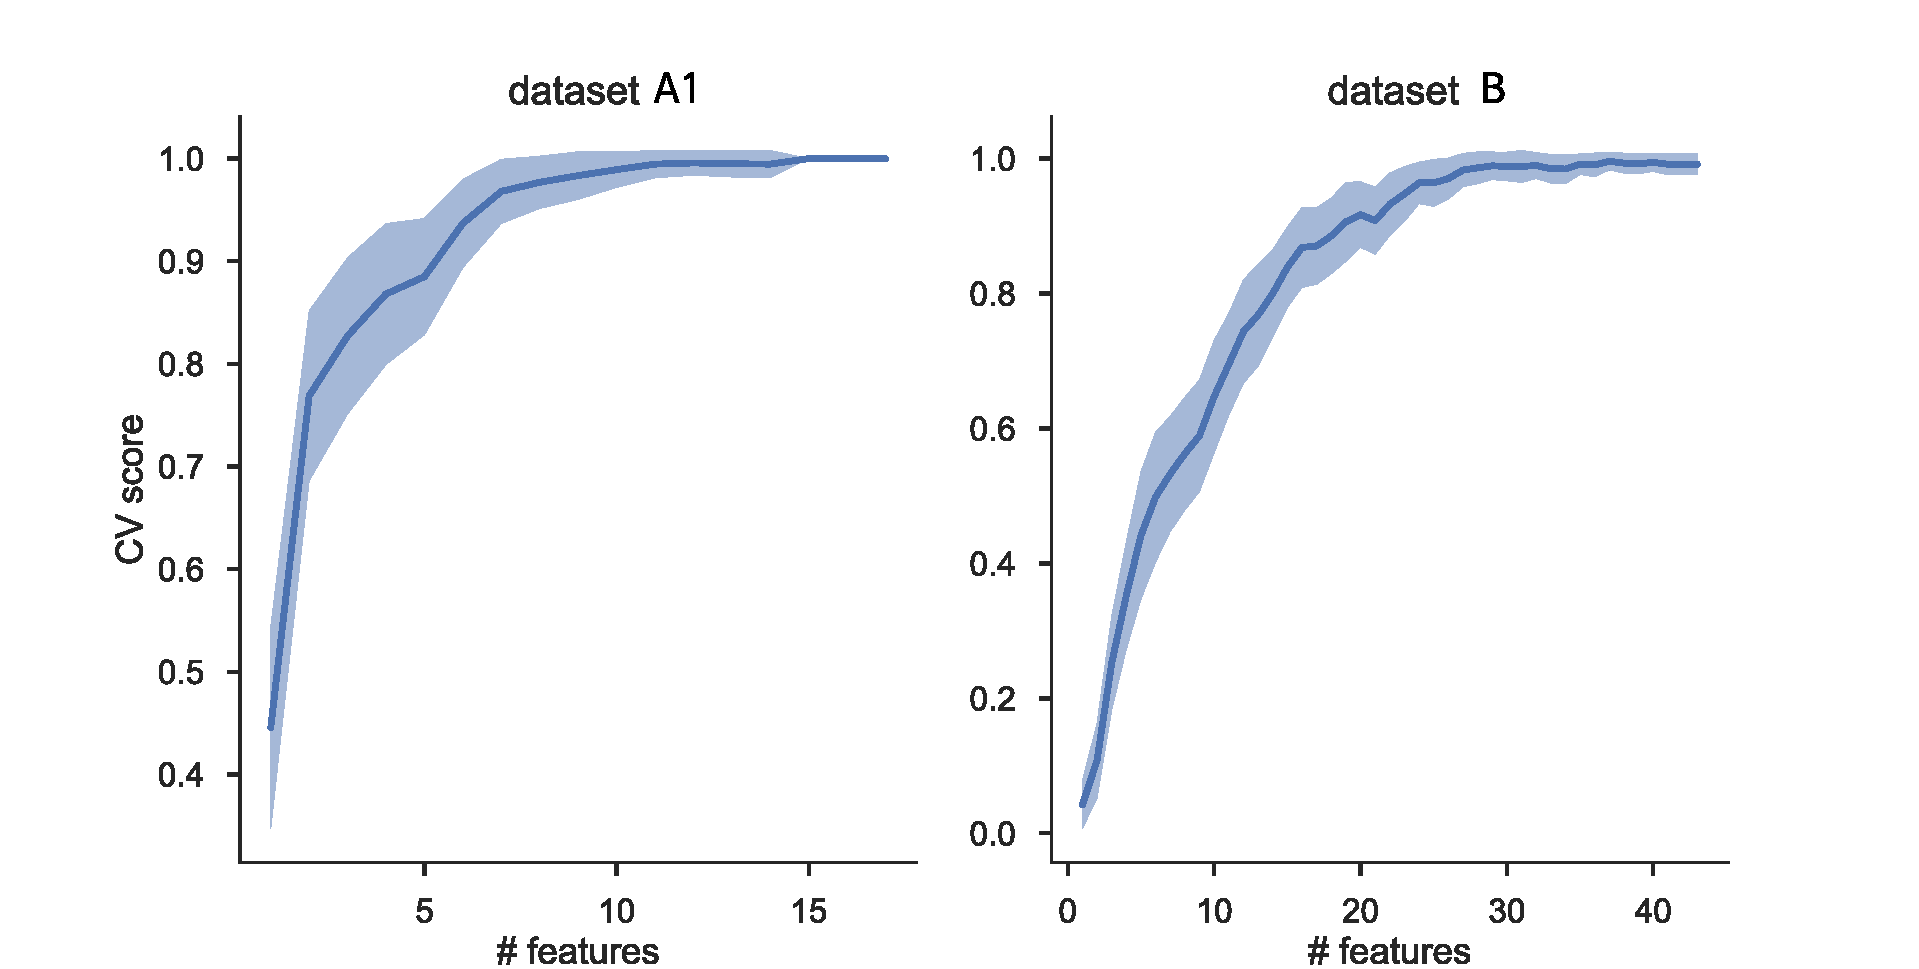
\includegraphics[width=0.8\columnwidth,valign=b]{subj_varying_links}
\end{center}
\end{frame}

\begin{frame}
\frametitle{Subjects classification}
\begin{center}
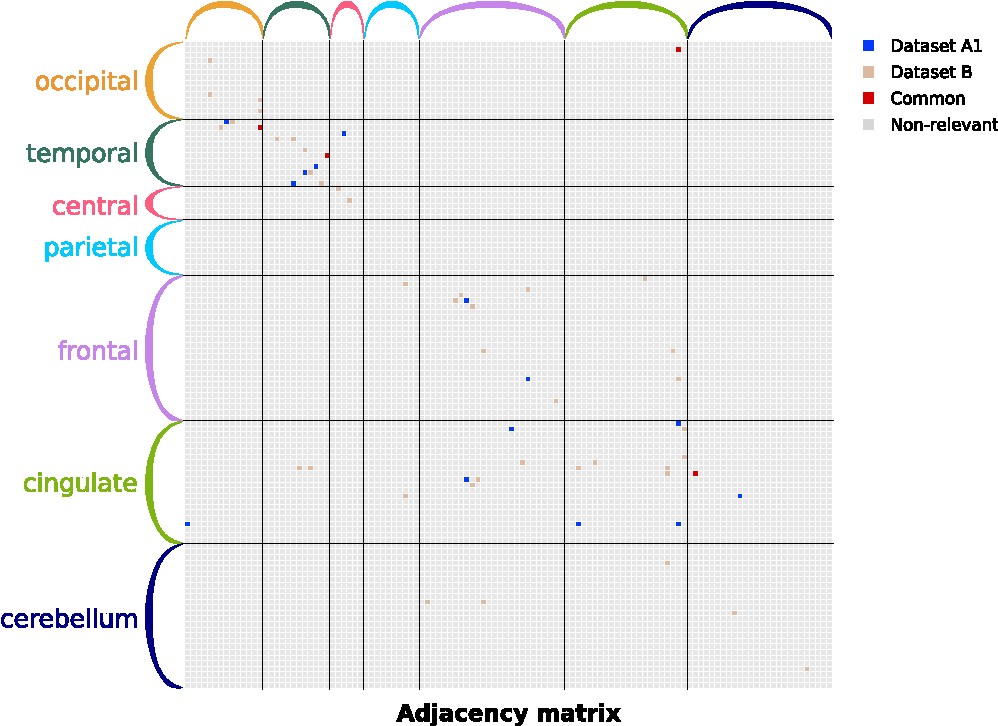
\includegraphics[width=0.8\columnwidth,valign=b]{subj_net}
\end{center}
\end{frame}

\begin{frame}
\frametitle{Subjects classification}
Average ranking by subsystem
\begin{center}
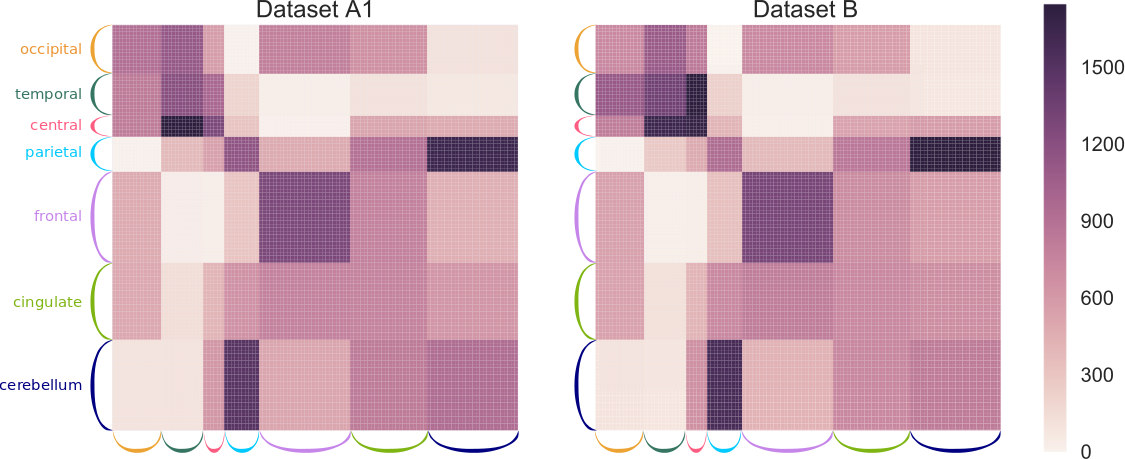
\includegraphics[width=0.8\columnwidth,valign=b]{avg_ranking_subsystems}
\end{center}
\end{frame}

\begin{frame}
\frametitle{Subjects classification}
Number of overlapping links is much higher than expected by chance
\begin{center}
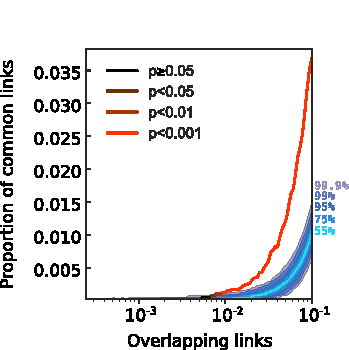
\includegraphics[width=0.5\columnwidth,valign=b]{subj_H0}
\end{center}
\end{frame}

\begin{frame}
\frametitle{Condition classification}
resting VS movie viewing

\pause
Classification accuracy using subsets of links according to RFE ranking
\begin{center}
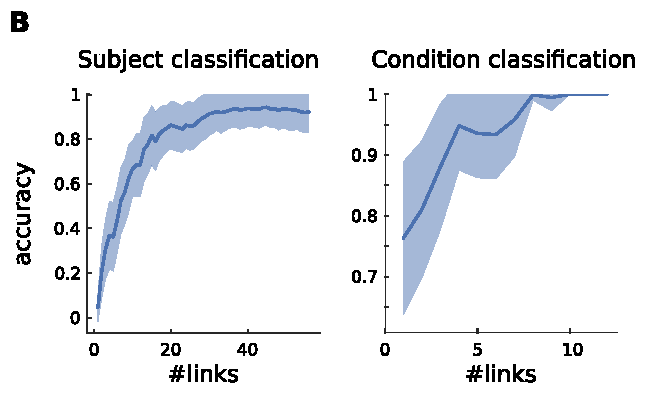
\includegraphics[width=0.8\columnwidth,valign=b]{subj_cond_results}
\end{center}
\end{frame}

\begin{frame}
\frametitle{Condition classification}
\begin{center}
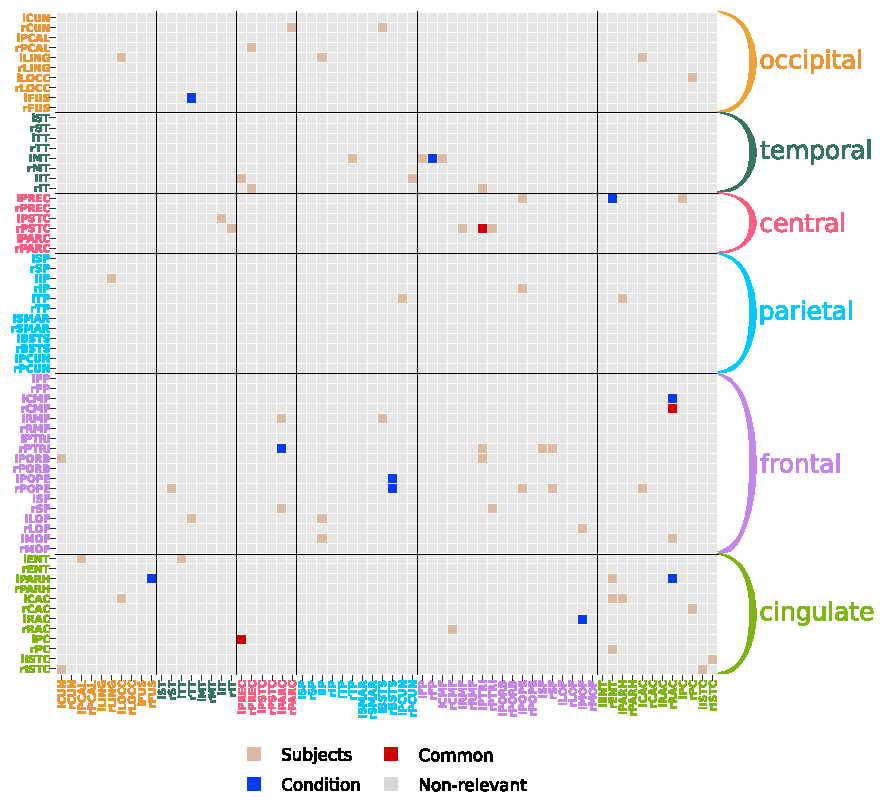
\includegraphics[width=0.65\columnwidth,valign=b]{subj_cond_matrix}
\end{center}
\end{frame}

\begin{frame}
\frametitle{Condition classification}
Number of overlapping links is similar to that expected by chance
\begin{center}
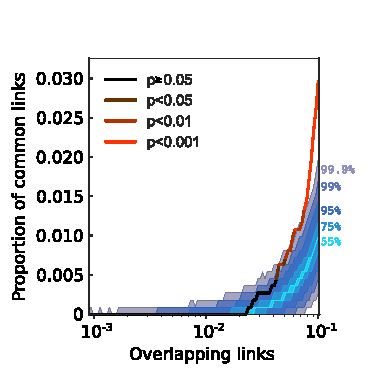
\includegraphics[width=0.5\columnwidth,valign=b]{cond_H0}
\end{center}
\end{frame}

\begin{frame}
\frametitle{Condition classification}
Subjects and conditions networks
\begin{center}
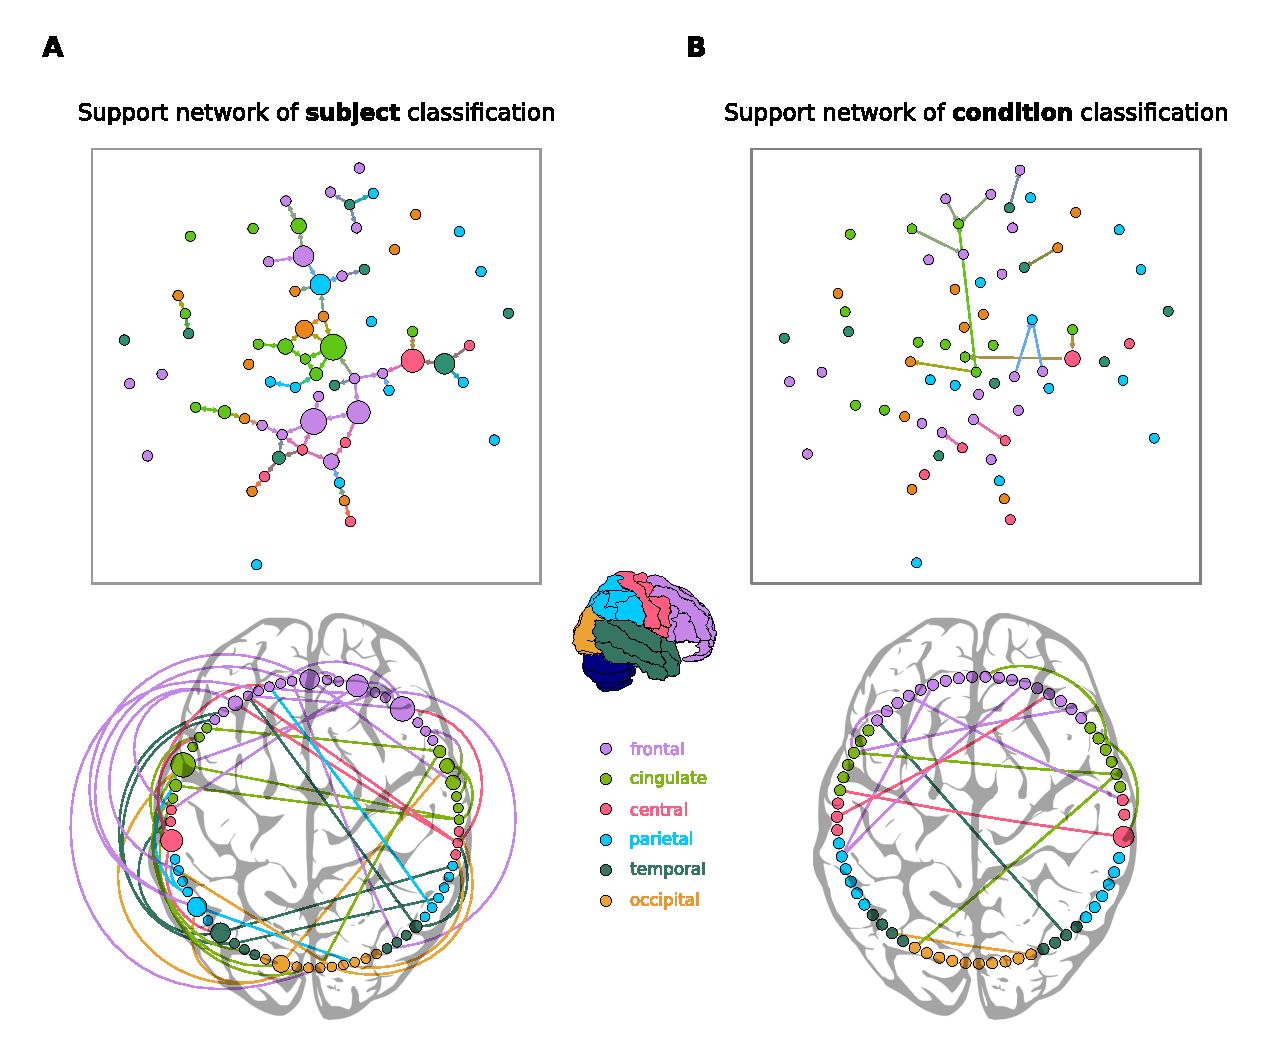
\includegraphics[width=0.7\columnwidth,valign=b]{fig5}
\end{center}
\end{frame}

\begin{frame}
	\frametitle{Summary (ad interim)}
	\begin{itemize}
		\item 
	\end{itemize}
\end{frame}

\begin{frame}
\frametitle{}
\centering
Estimation of parameters in the MOU model
\end{frame}

\begin{frame}
\transdissolve
\frametitle{Estimation of parameters}
\begin{itemize}
	\item Lyapunov optimization (Gilson et al. PLoS Comp Biol 2015)
	\item minimize $V = \sum_{m,n} (\mathbf{Q}_{mn}^0 - \mathbf{\hat{Q}}_{mn}^0)^2 +
		\sum_{m,n} (\mathbf{Q}_{mn}^{\tau} - \mathbf{\hat{Q}}_{mn}^{\tau})^2$
\end{itemize}
		\colortext{red}{Instert fig 2E matt paper}
\end{frame}

\begin{frame}
\transdissolve
\frametitle{Bayesian estimation of parameters}
\begin{itemize}
		\pause
	\item Posterior probability of parameters $\rightarrow$ connectivity estimation 
		\pause
	\item Regularization $\rightarrow$ better estimation with few timepoints
		\pause
	\item Model comparison 
\end{itemize}
\end{frame}

\begin{frame}
\transdissolve
\frametitle{Bayesian estimation of parameters}
\begin{itemize}
	\item Bayesian MAP estimate with uniform prior ($\equiv$ MLE): Tizio et al. 2017
	\item $C^* = logm[(\mathbf{Q^{0}})^{-1}\mathbf{Q^1}]
\end{itemize}
\end{frame}

\begin{frame}
\frametitle{MAP estimate for large scale networks}
\begin{center}
\includegraphics[width=0.7\columnwidth,valign=b]{}
\end{center}
\end{frame}

\begin{frame}
\frametitle{MAP estimate for small time samples}
\begin{center}
\includegraphics[width=0.7\columnwidth,valign=b]{}
\end{center}
\end{frame}

\begin{frame}
\frametitle{Influence of weight values}
\begin{center}
\includegraphics[width=0.7\columnwidth,valign=b]{}
\end{center}
\end{frame}

\begin{frame}
\frametitle{True and predicted weights}
\begin{center}
\includegraphics[width=0.7\columnwidth,valign=b]{}
\end{center}
\end{frame}

\begin{frame}
	\frametitle{Summary}
	\begin{itemize}
		\item 
	\end{itemize}
\end{frame}

\begin{frame}
\frametitle{Acknowledgments}
\begin{columns}
\begin{column}{0.5\textwidth}
\begin{center}
	\alert<2>{Vicente Pallares}\\
\vspace{1cm}

\alert<2>{Matthieu Gilson}\\
\vspace{1cm}

\small Ana Sanjuan\\
\vspace{0.5cm}

\small Simone Kuhn\\
\vspace{0.5cm}

\small Dante Mantini\\
\vspace{0.5cm}

\small Gustavo Deco\\
\vspace{0.5cm}

\normalsize John Cunningham\\
\end{center}
\end{column}
\begin{column}{0.5\textwidth}
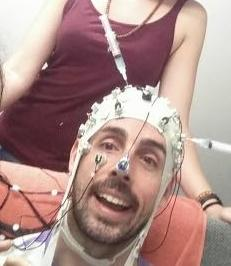
\includegraphics[width=0.5\columnwidth,valign=t]{vicente2}
\vspace{0.5cm}

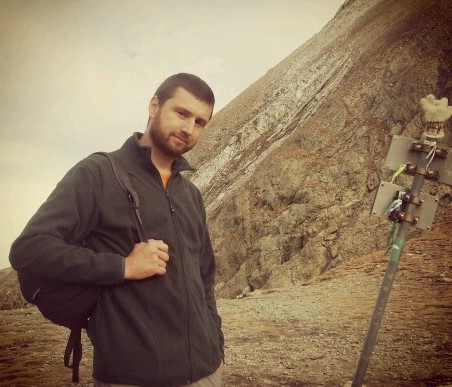
\includegraphics[width=0.5\columnwidth,valign=t]{matt}
\end{column}
\end{columns}
\end{frame}


\end{document}
